\section{计算空间距离}

\subsection{点到平面的距离}

\begin{theorem}
    点 $P$ 到平面 $A B C$ 的距离可以通过以下公式计算：
    \[
        d = \frac{|\overrightarrow{n} \cdot \overrightarrow{A P}|}{|\overrightarrow{n}|}
    \]
    其中，$\overrightarrow{n}$ 是平面的法向量，$\overrightarrow{A P}$ 是从平面上一点 $A$ 到点 $P$ 的向量。
\end{theorem}

\subsection{线面角与点面距的计算}

\begin{problem}
如图，在四棱柱 $A B C D-A_1 B_1 C_1 D_1$ 中，$A A_1 \perp$ 平面 $A B C D$ ，底面 $A B C D$ 是平行四边形，$A B=A D=B D=A A_1=2$ 。
\begin{enumerate}
    \item[(1)] 求直线 $B D_1$ 与平面 $A C D_1$ 所成角的正弦值；
    \item[(2)] 求点 $B_1$ 到平面 $A C D_1$ 的距离．
\end{enumerate}

\begin{figure} [H]
    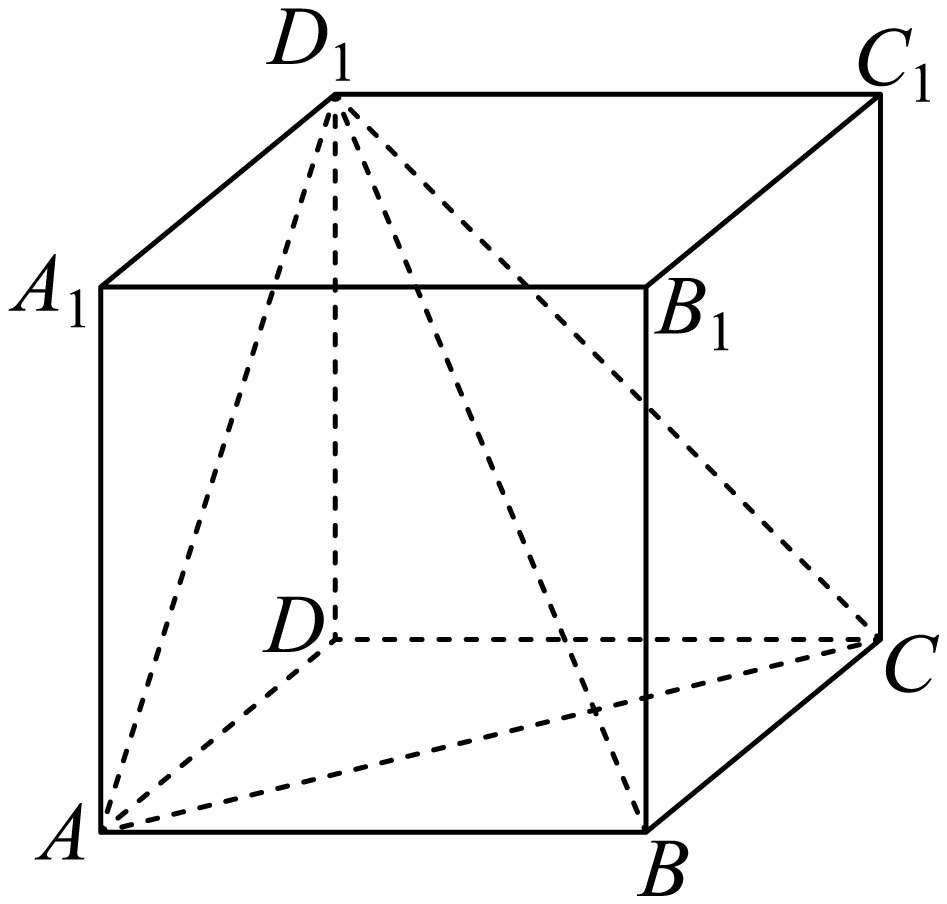
\includegraphics[width=0.2\textwidth]{chapters/立体几何/images/建系法求角/img-20250704221316.png}
\end{figure}

\end{problem}

\subsection{平行平面的距离}

\begin{theorem}
    以上，直接转化为点到平面的距离就能算了。
\end{theorem}

\begin{example}
    在棱长为 2 的正方体 $A B C D-A_1 B_1 C_1 D_1$ 中，求
    \begin{enumerate}
        \item 直线 $B C$ 与平面 $A B C_1 D_1$ 所成的角；
        \item 求平面 $A_1 B D$ 与平面 $B_1 D_1 C$ 的距离；
        \item 求三棱雉 $B_1-A_1 B D$ 外接球的表面积；
    \end{enumerate}
\end{example}

\begin{figure} [H]
    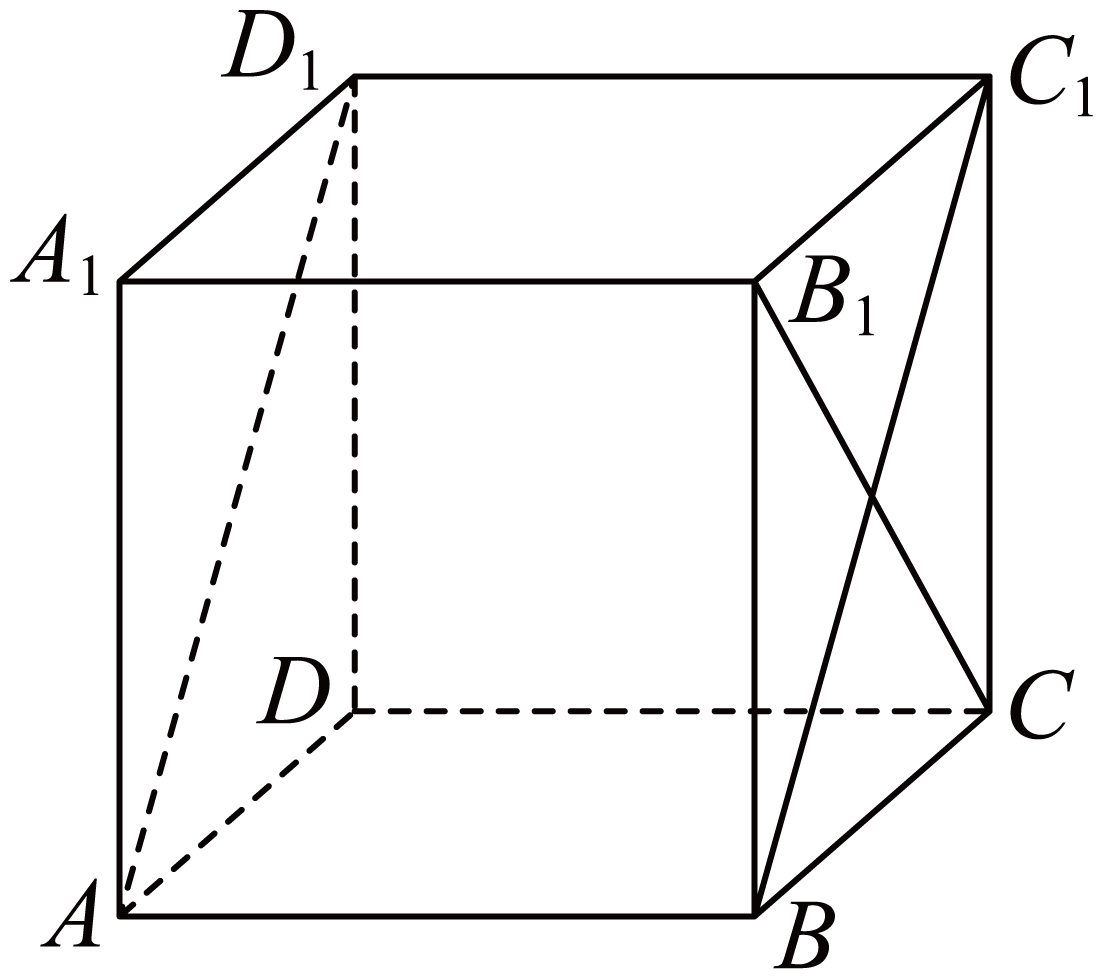
\includegraphics[width=0.2\textwidth]{chapters/立体几何/images/建系法求空间距离/img-20250824213808.png}
\end{figure}

\subsection{点到直线的距离}

\begin{theorem}

\end{theorem}

\subsection{异面直线的距离}

\begin{definition}
    两条异面直线之间的距离是指其中一条直线上任意一点到另一条直线距离的最小值。
\end{definition}

\begin{theorem}
    $AB$为异面直线 $a$、$b$ 的公垂线段，$\overrightarrow{n}$ 为直线$AB$的方向向量，$E$、$F$分别为直线 $a$、$b$ 上的任意一点，则
    \[
        |AB| = \frac{|\overrightarrow{EF} \cdot \overrightarrow{n}|}{|\overrightarrow{n}|}
    \]
\end{theorem}

\begin{figure}[h!]
    \centering
    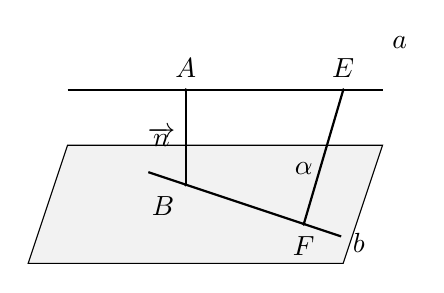
\begin{tikzpicture}[
            scale=1,
            >=stealth, % 箭头样式
            point/.style={circle, fill=black, inner sep=0.5pt} % 点的样式
        ]
        % 绘制平面 alpha
        \draw[fill=gray!10] (-2,0) -- (2,0) -- (2.5,1.5) -- (-1.5,1.5) -- cycle;
        \node at (1.5, 1.2) {$\alpha$};

        % 绘制直线 b 和 F, B 点
        \coordinate (F) at (1.5, 0.5);
        \coordinate (B) at (0, 1);
        \draw[thick, shorten <= -0.5cm, shorten >= -0.5cm] (B) -- (F);
        \node[point, label=below:$F$] at (F) {};
        \node[point, label=below left:$B$] at (B) {};

        % 绘制直线 a 和 E, A 点
        \coordinate (A) at (0, 2.2);
        \coordinate (E) at (2, 2.2);
        \draw[thick] (-1.5, 2.2) -- (2.5, 2.2);
        \node[above right] at (2.5, 2.6) {$a$};
        \node[below right] at (2, 0.5) {$b$};
        \node[point, label=above:$A$] at (A) {};
        \node[point, label=above:$E$] at (E) {};

        \draw[thick] (A) -- (B) node [midway, left] {$\overrightarrow{n}$};
        \draw[thick] (E) -- (F);

    \end{tikzpicture}
    \caption{异面直线公垂线段示意图}
    \label{fig:skew_lines}
\end{figure}

% --- 证明过程 ---
\begin{proof}
    显然 $\overrightarrow{AB} = \overrightarrow{AE} + \overrightarrow{EF} + \overrightarrow{FB}$，
    因为 $\overrightarrow{n}$ 是公垂线 $AB$ 的方向向量，所以 $\overrightarrow{n} \perp a$ 且 $\overrightarrow{n} \perp b$。
    又因为 $\overrightarrow{AE}$ 在直线 $a$ 上，$\overrightarrow{FB}$ 在直线 $b$ 上，所以 $\overrightarrow{AE} \perp \overrightarrow{n}$，$\overrightarrow{FB} \perp \overrightarrow{n}$。
    因此，它们的点积为零：
    \[ \overrightarrow{AE} \cdot \overrightarrow{n} = 0, \quad \overrightarrow{FB} \cdot \overrightarrow{n} = 0 \]
    所以，我们将 $\overrightarrow{AB}$ 与 $\overrightarrow{n}$ 作点积：
    \[
        \overrightarrow{AB} \cdot \overrightarrow{n} = (\overrightarrow{AE} + \overrightarrow{EF} + \overrightarrow{FB}) \cdot \overrightarrow{n}
    \]
    \[
        \overrightarrow{AB} \cdot \overrightarrow{n} = \overrightarrow{EF} \cdot \overrightarrow{n}
    \]
    两边取绝对值：
    \[
        |\overrightarrow{AB} \cdot \overrightarrow{n}| = |\overrightarrow{EF} \cdot \overrightarrow{n}|
    \]
    \[
        |AB| = \frac{|\overrightarrow{EF} \cdot \overrightarrow{n}|}{|\overrightarrow{n}|}
    \]
\end{proof}